\begin{figure}[h]
    \centering
    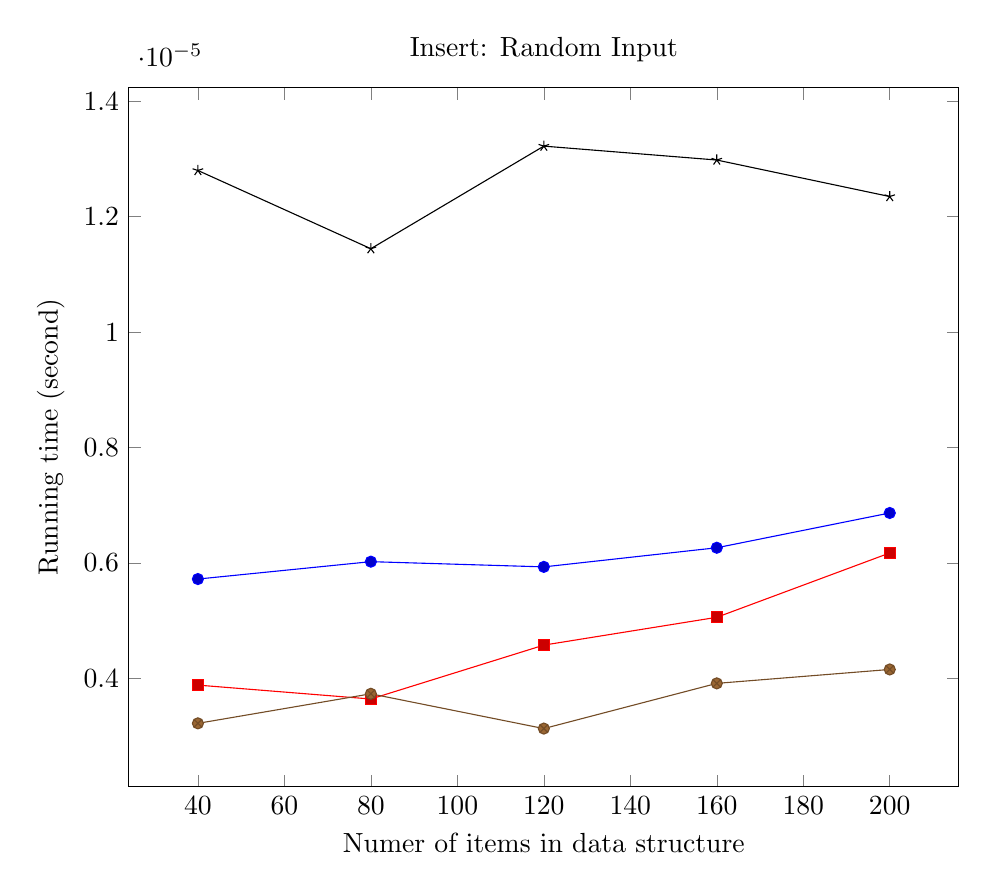
\begin{tikzpicture}
        \begin{axis}[
            xlabel={Numer of items in data structure},
            ylabel={Running time (second)},
            title={Insert: Random Input},
            width=\textwidth
        ]
		\addplot coordinates {
			(200, 6.866797677940184e-06)
			(160, 6.264447004433737e-06)
			(120, 5.933154134007967e-06)
			(80, 6.0235067350311585e-06)
			(40, 5.722331398280711e-06)
		};
		\addplot coordinates {
			(200, 6.174094403410546e-06)
			(160, 5.059745657429171e-06)
			(120, 4.57786511862679e-06)
			(80, 3.644221574694573e-06)
			(40, 3.885161844097151e-06)
		};
		\addplot coordinates {
			(200, 4.156219647175052e-06)
			(160, 3.915279377772473e-06)
			(120, 3.1322235022168686e-06)
			(80, 3.73457417572054e-06)
			(40, 3.2225761032428356e-06)
		};
		\addplot coordinates {
			(200, 1.2348188806818317e-05)
			(160, 1.298065701399731e-05)
			(120, 1.3221597283399888e-05)
			(80, 1.1444662796564199e-05)
			(40, 1.2799951811945375e-05)
		};
        \legend{}
        \end{axis}
    \end{tikzpicture}
    \caption{Average of 0 operations, benchmarked every 0, starting at 0.}
\end{figure}